\chapter{Aplicación web}
\label{chap:aplicacion_web}

\lettrine{U}{na} importante faceta de este proyecto es la forma en la que sirve para explicar el funcionamiento de un sistema paralelo, así como realizar demostraciones prácticas, tanto en directo como mediante vídeos, de dicho funcionamiento.

Para este cometido se desarrolla una aplicación web, el \textit{dashboard} de ahora en adelante, desde la cual se podrán ejecutar los benchmarks discutidos en el Capítulo \ref{chap:medida_rendimiento}. En este capítulo se discuten las etapas, desde el análisis hasta la implementación, y se proporcionan explicaciones sencillas acerca de su funcionamiento interno y externo.

Los archivos \LaTeX, scripts, imágenes y demás recursos relacionados con este trabajo, pueden encontrarse en la dirección \url{https://github.com/forcegk/GEI_TFG}. En especial, el dashboard tratado a lo largo de este capítulo se encuentra en la ruta \texttt{app/node}. 

\section{Requisitos}
Los principales requisitos del dashboard son los siguientes:

\begin{itemize}
    \item Debe ser \textbf{fácilmente accesible} y no debe \textbf{depender del sistema host}. Esto es, para acceder a dicha aplicación no se debe requerir un trabajo previo de media hora, así como realizar conexiones \acrshort{ssh}, etc. Debe ser una solución relativamente \textit{Plug-and-Play}.
    \item Debe ser \textbf{visualmente agradable} y \textbf{comprensible}. Además resultaría conveniente que la sección de monitorización resulte simple y vistosa, es decir, que no sea una masa de gráficas ininteligibles para el usuario con escasos conocimientos.
    \item Será \textbf{sencillo de utilizar} tanto para el usuario experimentado, como para el novato. No permitirá muchas operaciones desde la propia interfaz, pero será sencillo para el mantenedor agregar funcionalidad a la misma.
    \item Finalmente, debe estar \textbf{orientado} \textbf{a docencia y divulgación}, por lo que se deberá incluir contenido demostrativo en vídeo pregrabado y/o material interactivo para su uso en directo.
\end{itemize}

\section{Diseño}
\label{sec:contenido_didactico__diseño}
Para esta etapa se sigue un diseño basado en el propotipado, hasta dar con una solución que convenza al cliente. Tras ello, en la siguiente fase de implementación, se continúa ciclo de vida puramente incremental. En este caso dado que el cliente es la misma persona que el diseñador, se ha consultado a terceras personas para la obtención de críticas y otras aportaciones, especialmente desde el punto de vista de la funcionalidad, estética, y sencillez.

No se cuenta con versiones digitales de dichos \textit{mockups}, debido a que la mayoría surgen en un contexto de informalidad debido al trato con dichas terceras personas y, por tanto, son en papel escrito. Sin embargo, las ideas para implementar en la aplicación, por orden de ocurrencia son:

\begin{itemize}
  \item Implementación de un \textbf{sistema de monitorización interactivo} de Clúpiter.
  \item Refinamiento de la interactividad del anterior sistema, introduciendo la posibilidad de \textbf{ejecución de benchmarks}, así como de la \textbf{visualización} de su \textbf{salida por terminal} desde la propia aplicación.
  \item \textbf{Inclusión} de \textbf{dos vídeos} divulgativos o demostrativos. En concreto, se decide que el primero de ellos será divulgativo, con un estilo inspirador y didáctico, muy introductorio y dirigido a todo los públicos. El segundo vídeo se dirigirá a aquel público que muestre un interés mayor, ya que entrará en algo más de detalle, explicando superficialmente el funcionamiento de los superordenadores y \acrshort{mpi}.
  \item Sólo se programará para soportar \textbf{un usuario de forma concurrente}, ya que sería raro el caso en el que haya dos o más usuarios conectados, y tendría más bien poco sentido la ejecución simultánea de más de un benchmark.
\end{itemize}

Finalmente, una decisión de diseño muy importante es la de implementar dicha aplicación como web. Esto es así porque un navegador web es lo más cerca que se puede estar de \textit{cross-platform}, universalidad, y sencillez. Para acceder a la aplicación, hosteada en el propio clúster, únicamente debe obtenerse una dirección IP en rango y conectarse mediante el navegador de preferencia a la dirección del nodo maestro (que aloja la aplicación web). Así, independientemente de que el sistema desde el que se quiere exponer tenga un sistema operativo Windows, MacOS, Linux, Solaris, Haiku, o cualquier otro sistema exótico, será suficiente con que éste tenga un navegador web con soporte JavaScript.

\section{Implementación}
La tecnología sobre la que se programa el \textit{\gls{backend}} de la aplicación web es nodejs, en concreto expressjs\footnote{\url{https://expressjs.com/es/}}, y se hace uso de las \acrshort{api}s de Netdata y socket.io.

La elección de socket.io se realiza debido a la sencillez y elegancia que aporta al código, el cual se puede programar mediante ``eventos''. Esto es algo fantástico, ya que desde la propia aplicación web se pueden hacer llamadas al \textit{\gls{backend}} con el mismo estilo de programación que en Android, resultando familiar y sencillo.

La página de monitorización es la única que se comunica con Clúpiter. Desde esta página se pueden ejecutar cada uno de los benchmarks (en clase \texttt{C}), y observar su salida por terminal, así como ver en tiempo real el impacto que la ejecución de los mismos tiene sobre la carga en los nodos.

\subsection{Comunicación socket.io}
\label{ssec:socket.io_comm}
La página web de socket.io contiene una fantástica documentación, pero se va a poner un ejemplo sencillo de cómo se emplea su funcionalidad para el dashboard: el proceso de comunicación para la ejecución de un benchmark.

\begin{enumerate}
  \item Al iniciar la página del dashboard, el cliente se conecta mediante un \textit{socket} al servidor. Esta conexión se realiza con una línea:
\begin{lstlisting}[language=java]
var socket = io();
\end{lstlisting}
  \item Cuando el usuario hace click en un botón, se llama a la siguiente función:
\begin{lstlisting}[language=java]
function spawn(bench_name) {
    toggleButtonActivation(true);
    socket.emit('spawn', bench_name);
}
\end{lstlisting}
  \item El servidor, que se encuentra esperando, comprueba la validez del comando recibido para evitar ataques \textit{shell/command injection} o similares, y emite de vuelta la salida del comando a ejecutar:
\begin{lstlisting}[language=java]
io.on('connection', (socket) => {
    // Cuando se recibe el evento spawn
    socket.on('spawn', (bench_name) => {
        console.log('User ' + socket.id + ' called benchmark: ' + bench_name);

    // Se procesa y comprueba [...]

    // Y se ejecuta el comando, redirigiendo stdout al dashboard
    const cmd = spawn(command, params, {shell:true});
    cmd.stdout.on('data', (data) => {
        socket.emit('youve_got_mail', utf8.encode(data.toString()));
    });
\end{lstlisting}
  \item El cliente web recibe un mensaje por el socket con el nombre `\texttt{youve\_got\_mail}', el cual incluye un dato \texttt{(msg)}, que se pasará a la función:
\begin{lstlisting}[language=java]
socket.on('youve_got_mail', (msg) => addTextToTextArea(msg));
\end{lstlisting}
  \item El servidor, cuando se termina de ejecutar el benchmark, recibe el evento \texttt{'close'}, y envía el mensaje \texttt{'finished\_execution'}:
\begin{lstlisting}[language=java]
cmd.stdout.on('close', (code) => {
    socket.emit('finished_execution', utf8.encode(`Program exited with code ${Number(code)}`));
});
\end{lstlisting}
  \item Dicho mensaje lo recibe también el cliente, que procede de la forma deseada:
\begin{lstlisting}[language=java]
socket.on('finished_execution', function(msg) {
    toggleButtonActivation(false);
    addBlankLineToTextArea();
    addBlankLineToTextArea();
    addTextToTextArea(msg);
    addBlankLineToTextArea();
    addBlankLineToTextArea();
});
\end{lstlisting}
\end{enumerate}

\subsection{Modularidad}
Un punto fuerte de esta implementación de terminal es que puede ejecutar cualquier comando de forma segura con poco trabajo y redirigir su salida estándar a la web. Se pone el ejemplo de la implementación de un botón de apagado de Clúpiter:

\begin{enumerate}
  \item Se añade el botón, su estilo y su comportamiento.
  \item En la función onClick se llama con la función \texttt{spawn(event)} al evento que se desea ejecutar:
\begin{lstlisting}[language=java]
spawn('poweroff');
\end{lstlisting}
  \item El backend recibe el evento y lo procesa con la siguiente sentencia switch, a la que se añade el caso `poweroff':
\begin{lstlisting}[language=java]
switch (bench_name) {
    case 'lu':
    case 'cg':
    case 'ft':
    case 'is':
    case 'mg':
    case 'ep':
        command = 'mpirun';
        params = ['-np', '32', '--hostfile', '/mpishared/hostfile', '--mca', 'opal_warn_on_missing_libcuda', '0', `/mpishared/NPB3.4.2/NPB3.4-MPI/bin/${bench_name}.*.x`];
        break;

    case 'poweroff':
        command = '/usr/local/bin/clupiter_poweroff';
        params = [];
        break;
    
    // [...]
}
\end{lstlisting}
  \item Finalmente, el comando junto con sus argumentos se ejecuta, y la salida estándar se redirige a la interfaz web, como se explica en la sección anterior (\ref{ssec:socket.io_comm}).
\end{enumerate}

\section{Vídeos didácticos}
\label{sec:videos_didacticos}
Como se comenta en la Sección \ref{sec:contenido_didactico__diseño}, se graban dos vídeos didácticos y divulgativos. El primero de ellos trata de manera muy superficial el concepto de superordenador, se aporta contexto histórico y cifras acerca de lo enorme de estas máquinas de cómputo, y cuales son y han sido sus utilidades y logros. Tras ello se realiza una descripción de Clúpiter y sus partes fundamentales, y se relacionan con sus análogos en un supercomputador real. Este vídeo está claramente orientado a educar en conceptos muy básicos acerca del \acrshort{hpc}, pero también a motivar e inspirar a futuros ingenieros. El vídeo en cuestión puede encontrarse en la dirección \url{https://youtu.be/o76-VP6WFCo}.

El segundo vídeo, ya más técnico, habla mediante animaciones ilustradas a mano acerca del funcionamiento interno de un supercomputador, su necesidad en el día a día, y las restricciones que tienen que superar los programas paralelos, mediante analogías y evitando el tecnicismo. Tras ello, se da una breve introducción a las operaciones más básicas de \acrshort{mpi}, y se finaliza el vídeo con una cuestión acerca de cómo ordenar diez mil hojas a mano entre varias personas, un recurso que expositor podrá emplear si lo considera conveniente. Con esta tarea se pueden explicar de manera intuitiva, e incluso competiva, múltiples conceptos de computación. En concreto se pueden razonar los algoritmos de ordenación y visualizar de primera mano las restricciones de la programación paralela, incluyendo la ralentización que supone el acceso a red, o las diferencias de acceso a memoria uniforme (\acrshort{uma} o \acrlong{uma}) con respecto al no uniforme (\acrshort{numa} o \acrlong{numa}). Dicho vídeo se puede encontrar en la dirección \url{https://youtu.be/if0MWI_9xzM}.

Finalmente, destacar que estos vídeos, en su versión alojada en YouTube, cuentan con subtítulos en español en caso de que sean expuestos a personas con discapacidades auditivas.

\section{Despliegue}
En esta sección se muestran los comandos a ejecutar para el despliegue y configuración del dashboard y sus dependencias.

\subsection{Instalación de Netdata}
Netdata es un software de monitorización de fácil configuración e integración que permite obtener información de los nodos de Clúpiter en tiempo real, tanto en el dashboard web que se pone a disposición del usuario en el puerto 19999, como a través de la librería JavaScript que un programador puede importar en su propia página web.

Para emplear los datos que proporciona este software, primero debe instalarse y activarse en cada uno de los nodos del clúster, acción que se realiza con los siguientes comandos, ejecutados como usuario \texttt{root}:

\begin{lstlisting}[language=bash]
pacman -S netdata   # Se instala netdata
# Se activa netdata a través de todas las interfaces
sed -i 's/bind to = localhost/bind to = 0.0.0.0/g' /etc/netdata/netdata.conf
# Se activa e inicia netdata
systemctl enable --now netdata
\end{lstlisting}

\subsection{Instalación del dashboard}
Para desplegar el dashboard es necesario instalar npm y git en el nodo maestro. Git se instala debido a que se clonará el repositorio de recursos de Clúpiter enlazado previamente en el inicio de este mismo capítulo.
\begin{lstlisting}[language=bash]
pacman -S npm git --needed      # como root
\end{lstlisting}

Tras ello se procede a desplegar la aplicación web:
\begin{lstlisting}[language=bash]
# Se crea el directorio /clupiter_dashboard y se le dan permisos a mpiuser
mkdir -p /clupiter_dashboard
chown -R mpiuser:mpiuser /clupiter_dashboard

# Se inicia sesión como mpiuser
su - mpiuser
cd /clupiter_dashboard

# Se descarga la app y se entra al directorio del servidor
git clone https://github.com/forcegk/GEI_TFG.git
cd GEI_TFG/app/node/

# Se instalan las dependencias
npm install --only=production

# Se juntan los trozos de vídeo
cat www/video/vid_1.mp4__* > www/video/vid_1.mp4

# Y se ejecuta manualmente una vez para probar con
node ./index.js
\end{lstlisting}

Si todo ha funcionado correctamente se podrá acceder a la página principal del dashboard en la dirección web \url{http://192.168.0.220:3000}.\footnote{Si se desea actualizar el software debería ser suficiente con realizar \texttt{git pull}. En caso de error, lo más cómodo es simplemente eliminar el directorio del dashboard con \texttt{rm -rf /clupiter\_dashboard} y ejecutar estos comandos de nuevo. En cualquier caso, tras la actualización es conveniente reiniciar la unidad de systemd.} 

Desde ella se podrá acceder a todas las páginas del dashboard: la de inicio, monitorización y el acerca de. En la página de inicio (Figura \ref{fig:inicio_clupiter}) se muestran los dos videos divulgativos de los que se ha hablado en la Sección \ref{sec:videos_didacticos}. En la página de monitorización (Figura \ref{fig:pagina_monitorizacion}) se encuentran los medidores de uso de CPU y tráfico de red de cada uno de los nodos. Estos medidores son los que se utilizaron en el capítulo anterior para estudiar el comportamiento de los NPB (Figuras \ref{fig:mops__cg}\textasciitilde\ref{fig:mops__mg}). Debajo de los mismos se encuentran botones para ejecutar cada uno de los benchmarks. En la pagina de ``acerca de'' (Figura \ref{fig:acercade_clupiter}) se incluye una breve descripción de Clúpiter y los agradecimientos. 

\begin{figure}[h!]
  \centering
  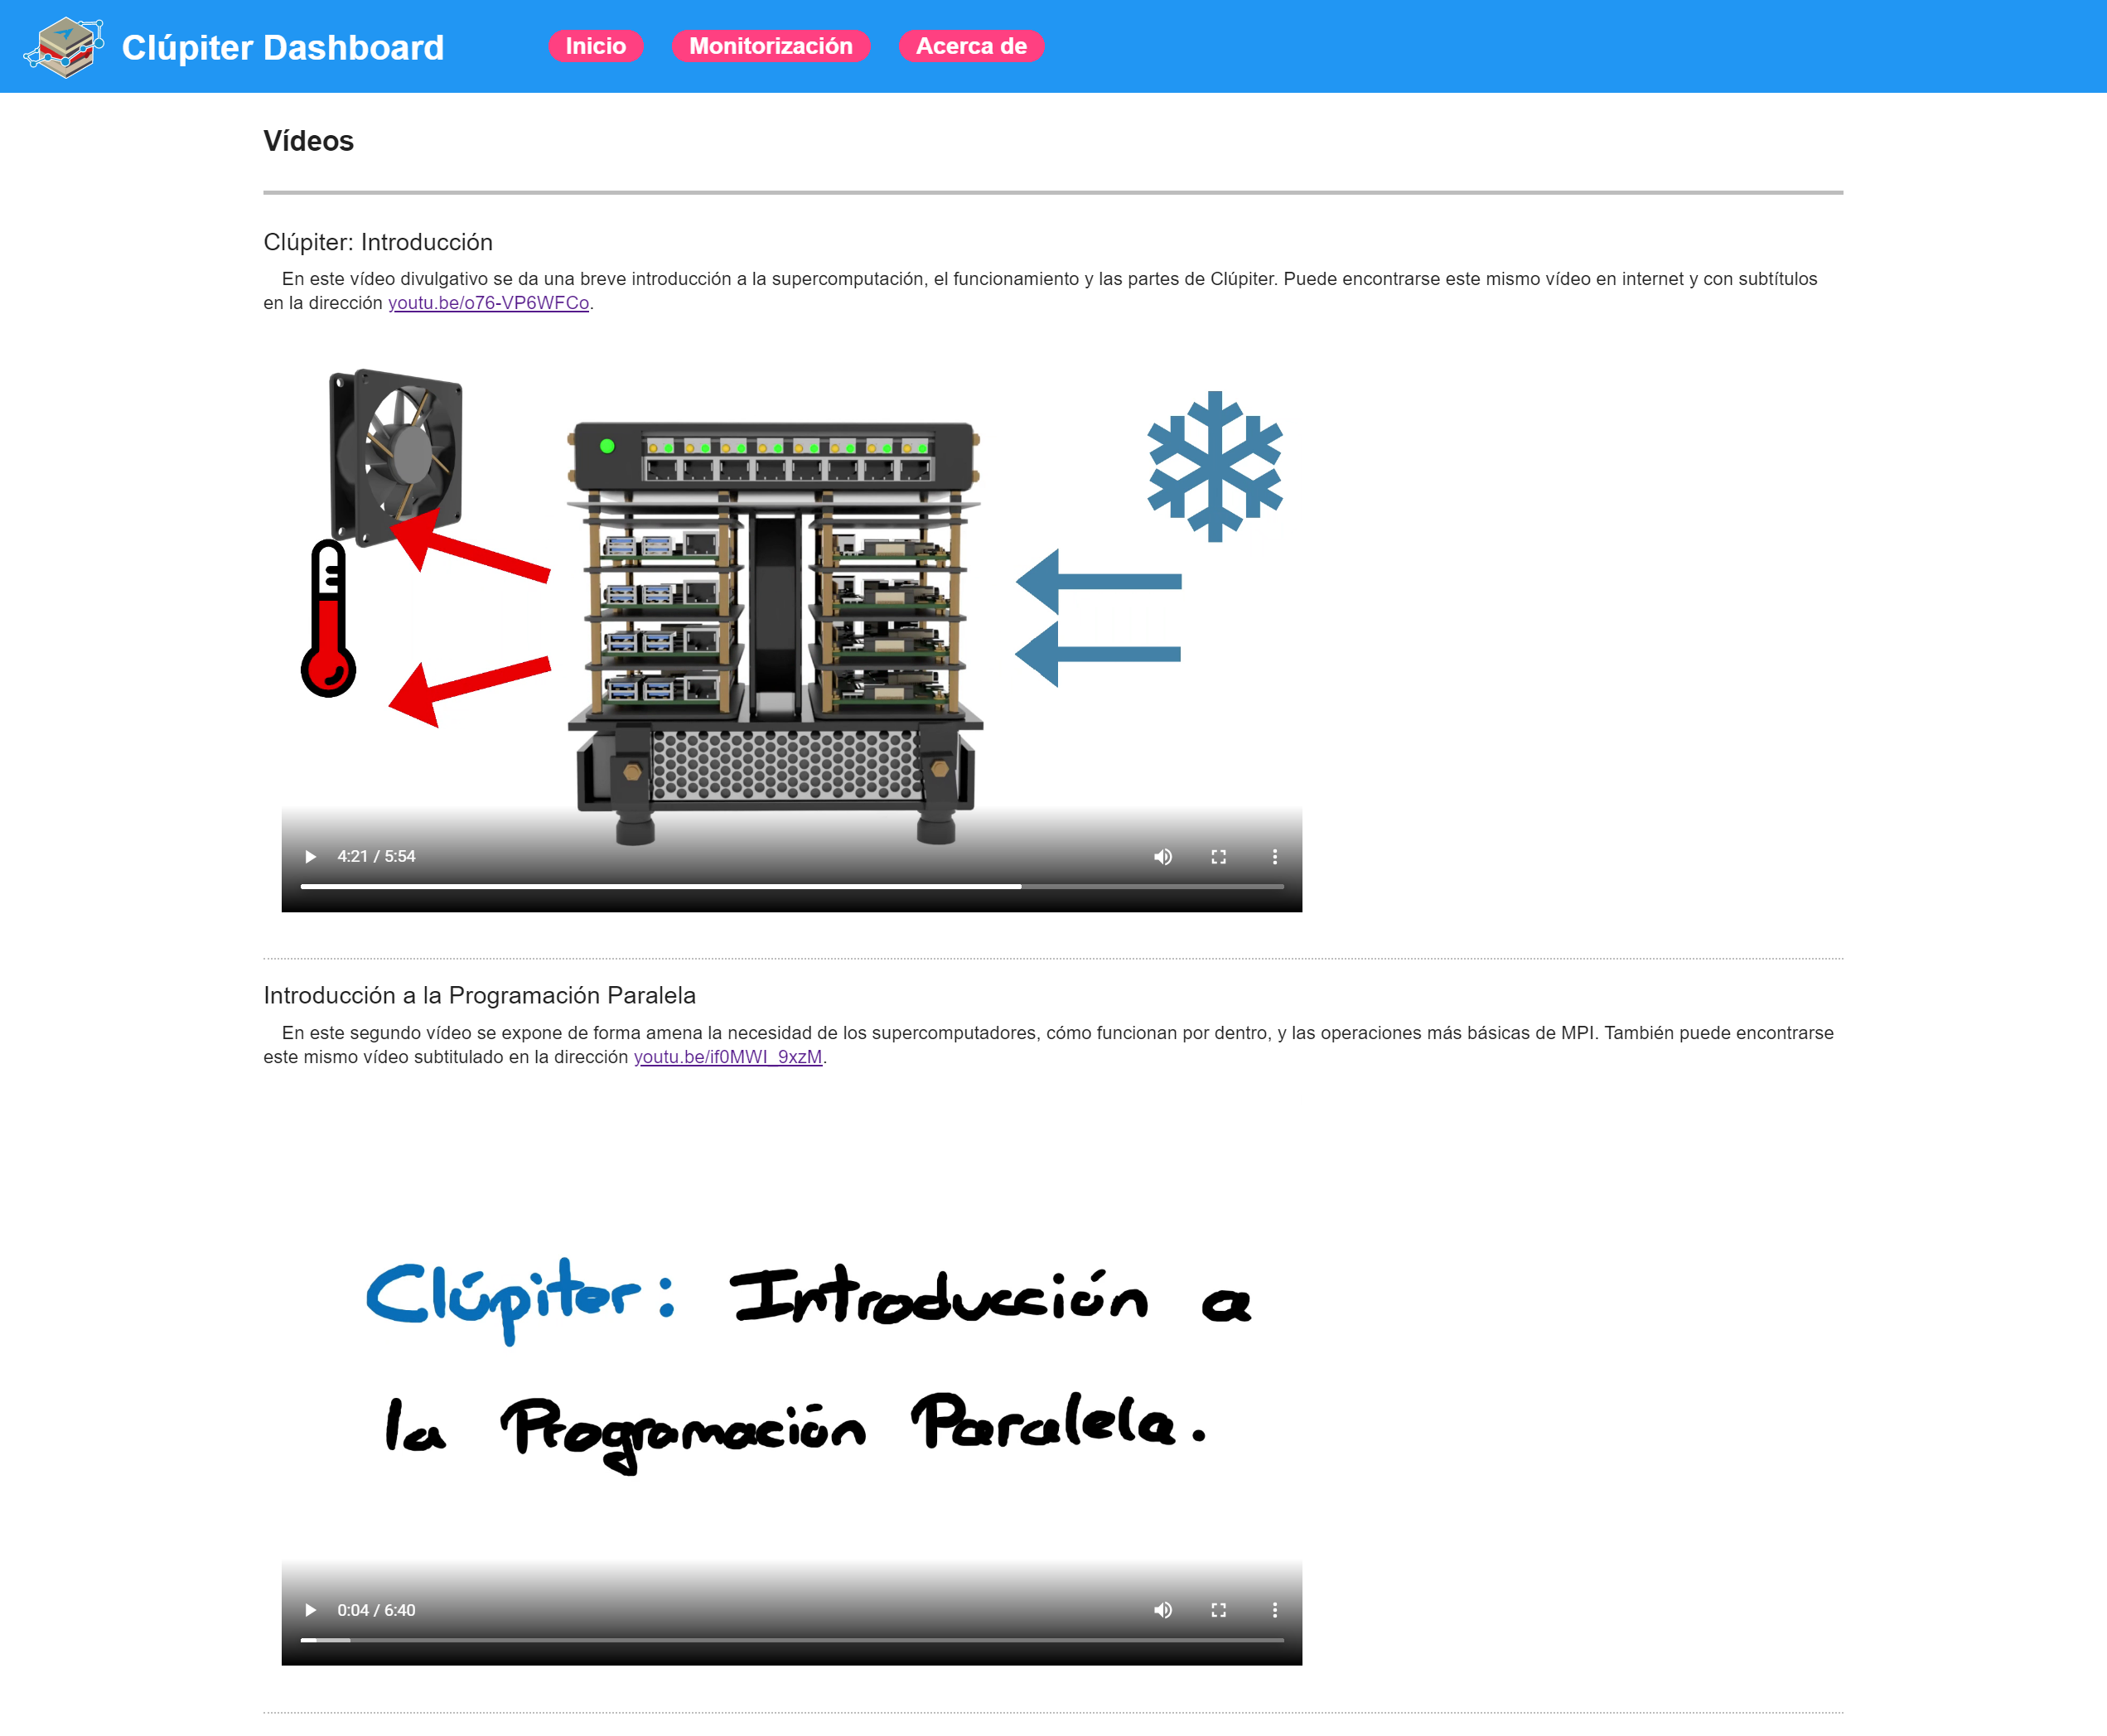
\includegraphics[width=0.9\textwidth]{img/dashboard/inicio.png}
  \caption{Página de inicio de Clúpiter}
  \label{fig:inicio_clupiter}
\end{figure}

\begin{figure}[h!]
  \centering
  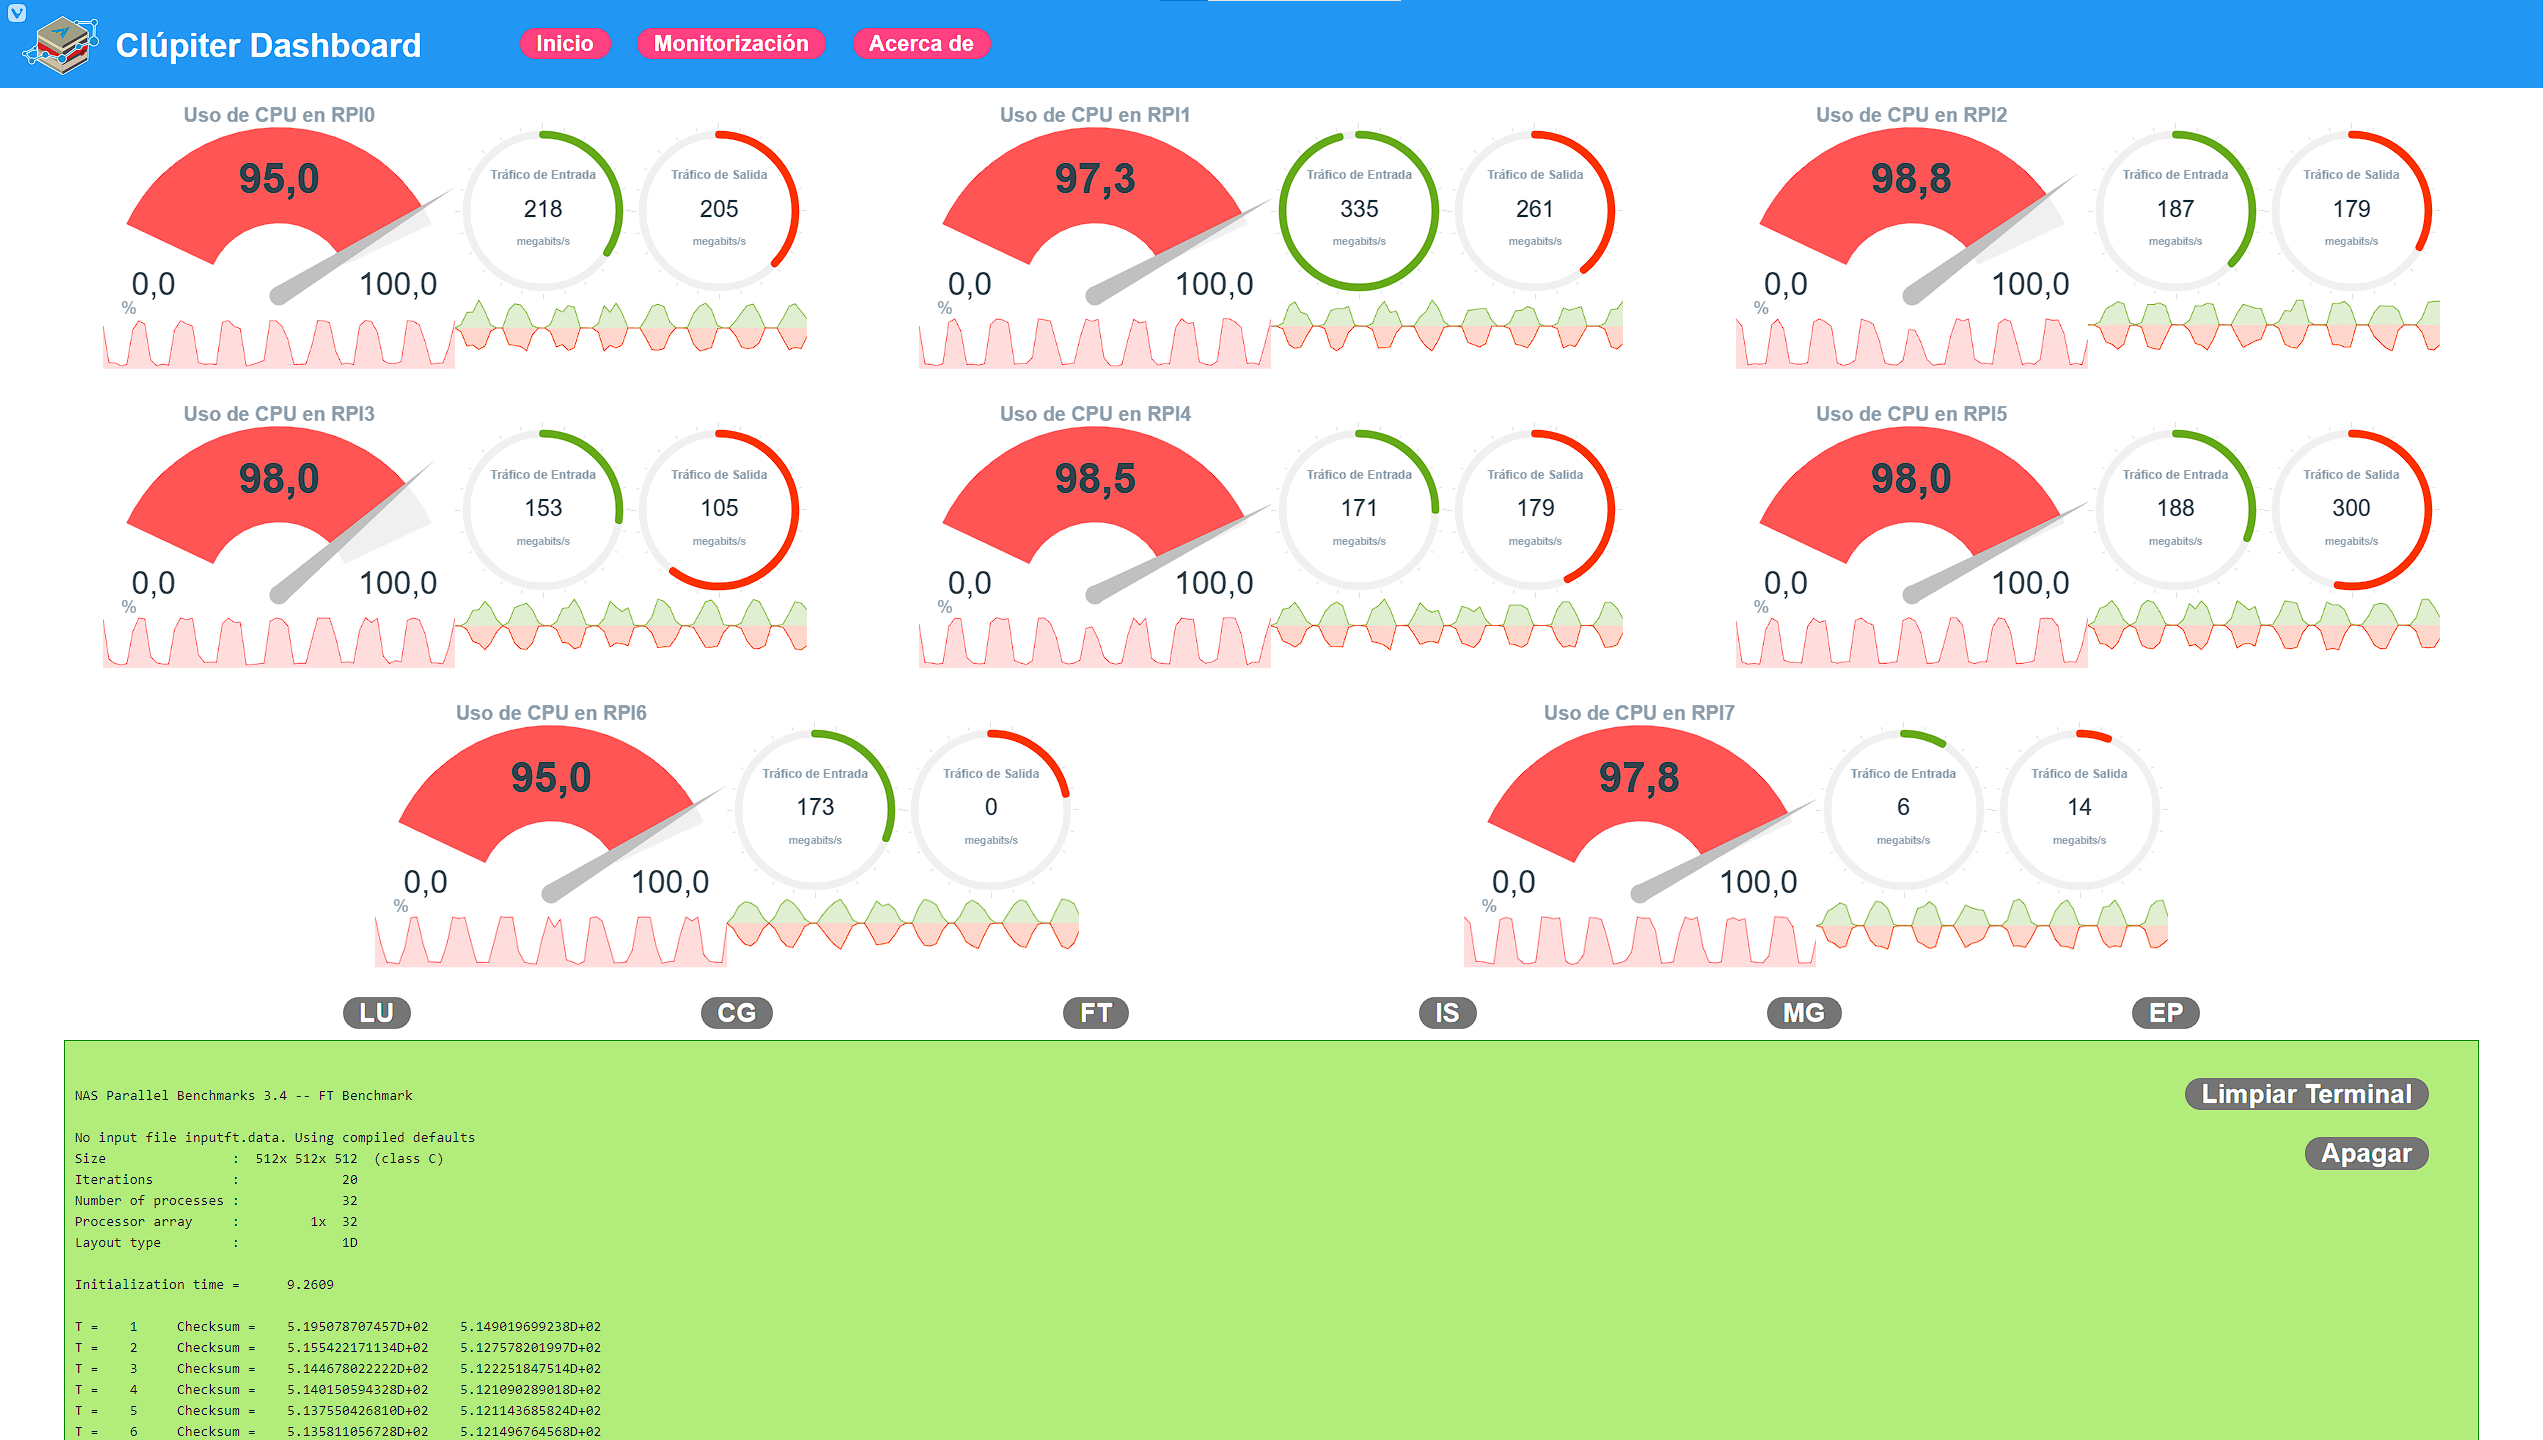
\includegraphics[width=0.95\textwidth]{img/dashboard/monitoring.png}
  \caption{Página de monitorización de Clúpiter}
  \label{fig:pagina_monitorizacion}
\end{figure}

\begin{figure}[h!]
  \centering
  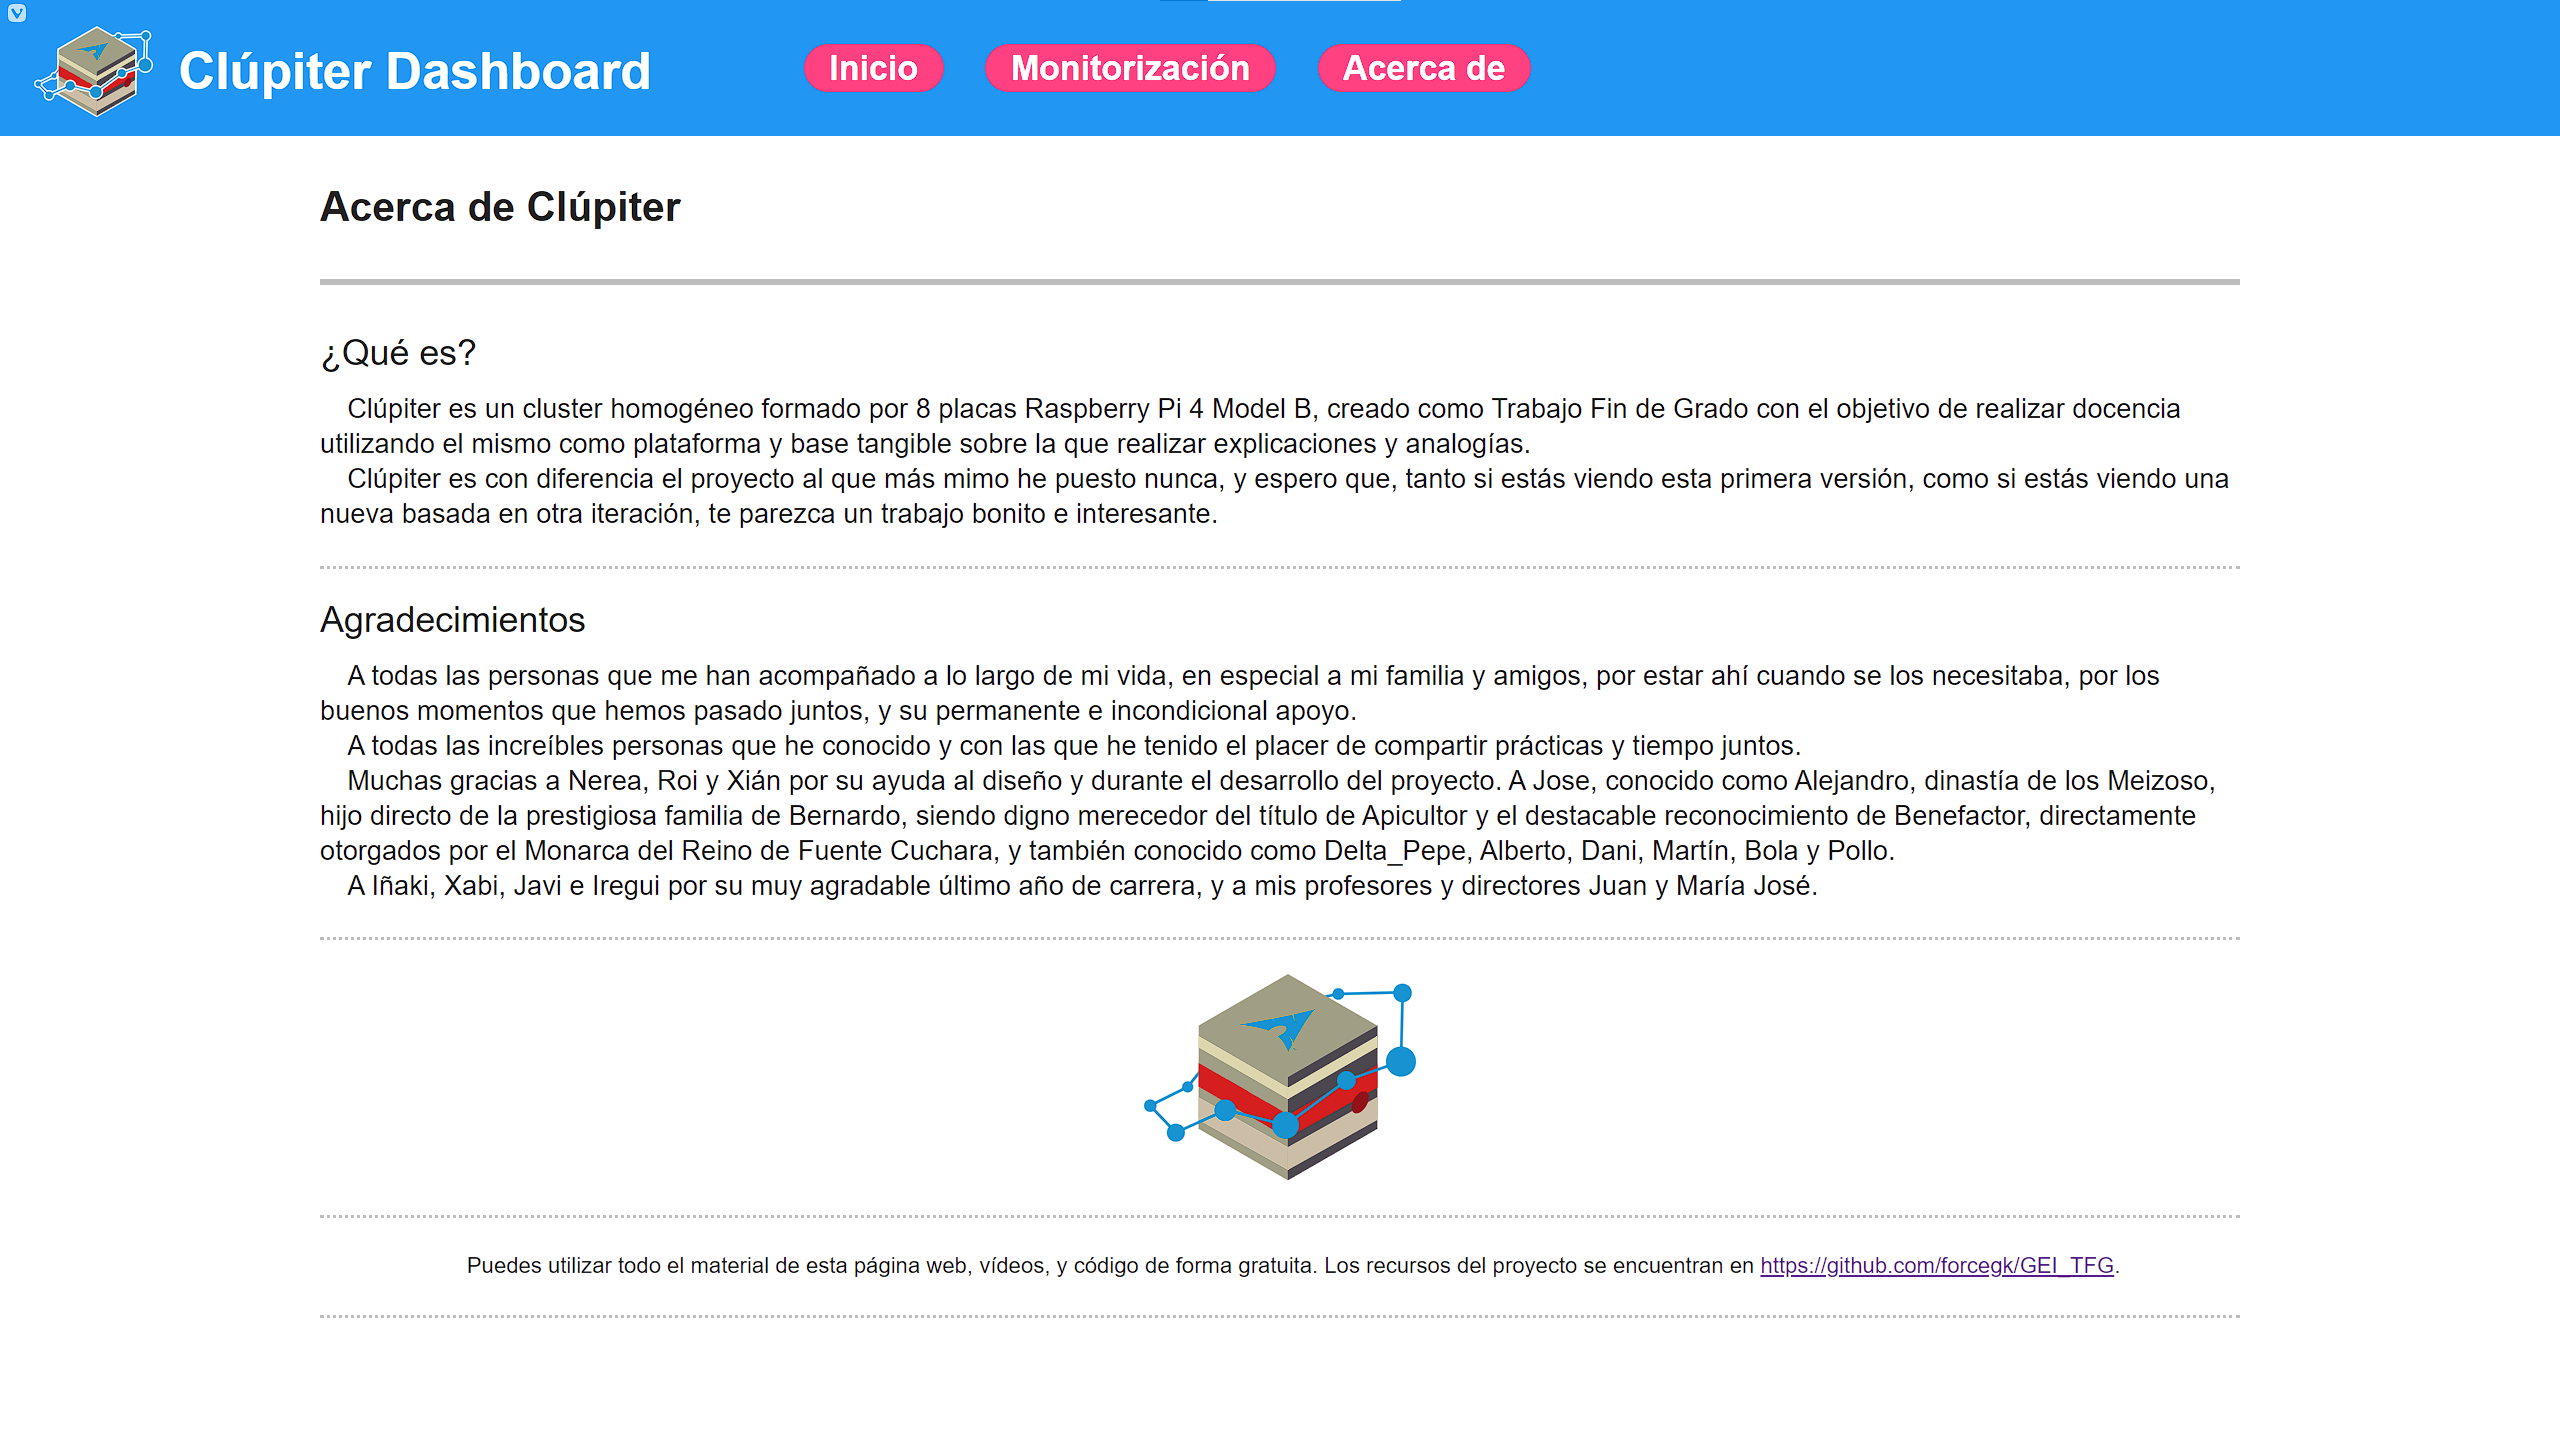
\includegraphics[width=0.9\textwidth]{img/dashboard/agradecimientos.png}
  \caption{Página ``acerca de'' de Clúpiter}
  \label{fig:acercade_clupiter}
\end{figure}
\FloatBarrier
\subsection{Creación de unidad de systemd}
Crear una unidad (o \textit{unit}) de systemd es necesario para que el dashboard se inicie con el nodo maestro. Realizar esto es una operación moderadamente sencilla (si bien no tan sencilla como podría ser en otros sistemas de init\footnote{\url{https://wiki.gentoo.org/wiki/Comparison_of_init_systems}}). 

La creación de la unidad se realiza editando como usuario \texttt{root} el fichero \texttt{/etc/systemd/system/clupiter\_dashboard.service}:

\begin{lstlisting}[]
[Unit]
Description=Service for Clupiter Dashboard
After=network.target

[Service]
Type=simple
User=mpiuser
WorkingDirectory=/clupiter_dashboard/GEI_TFG/app/node
ExecStart=/usr/bin/node /clupiter_dashboard/GEI_TFG/app/node/index.js
Restart=on-failure

[Install]
WantedBy=multi-user.target
\end{lstlisting}

Tras la creación de la unidad, se recarga el demonio de systemd, y se inicia el dashboard, también como \texttt{root}:
\begin{lstlisting}[language=bash]
# Se reinicia el demonio
systemctl daemon-reload

# Se activa e inicia el servicio
systemctl enable --now clupiter_dashboard.service

# Se puede verificar el correcto inicio del servicio con
systemctl status clupiter_dashboard.service
\end{lstlisting}

Si todo ha funcionado correctamente, se debería ver la pantalla mostrada en la Figura \ref{fig:systemd_clupiter_dashboard} al ejecutar el último comando (de la cual se puede salir presionando la letra \texttt{q}).

\begin{figure}[h!]
  \centering
  \vspace*{0.5cm}
  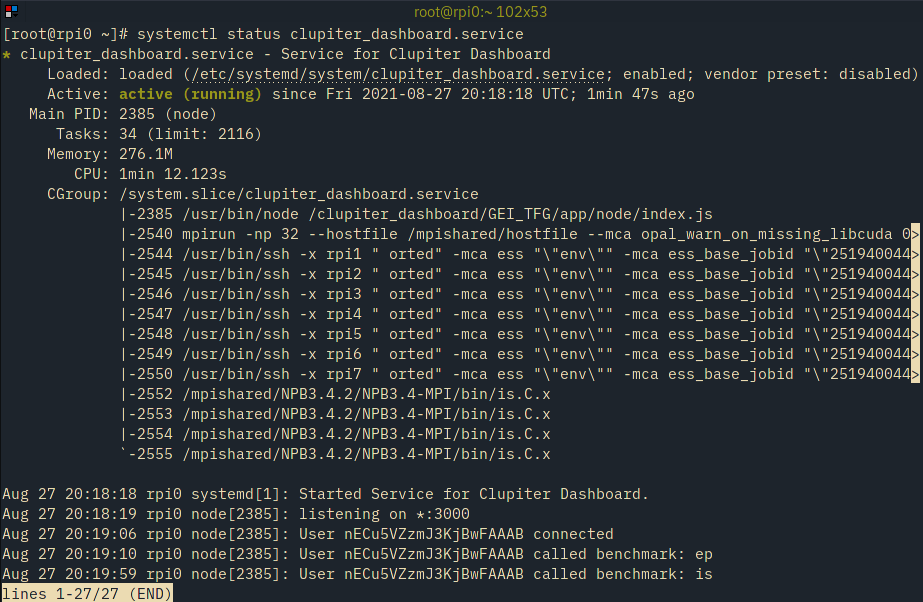
\includegraphics[width=0.9\textwidth]{img/systemd_clupiter_dashboard.png}
  \caption{Servicio \textit{Clupiter Dashboard} ejecutando un benchmark correctamente}
  \label{fig:systemd_clupiter_dashboard}
\end{figure}

% TODO IMAGEN DEL DASHBOARD
